\documentclass{article}%
\usepackage[T1]{fontenc}%
\usepackage[utf8]{inputenc}%
\usepackage{lmodern}%
\usepackage{textcomp}%
\usepackage{lastpage}%
\usepackage[head=40pt,margin=0.5in,bottom=0.6in]{geometry}%
\usepackage{graphicx}%
%
\title{\textbf{ONU libera 9,2 millones de dólares para atención médica y nutrición en Venezuela}}%
\author{AFP}%
\date{26/11/2018}%
%
\begin{document}%
\normalsize%
\maketitle%
\textbf{URL: }%
http://www.eluniversal.com/venezuela/26809/onu{-}libera{-}92{-}millones{-}para{-}atencion{-}medica{-}y{-}nutricion{-}de{-}venezuela\newline%
%
\textbf{Periodico: }%
EU, %
ID: %
26809, %
Seccion: %
venezuela\newline%
%
\textbf{Palabras Claves: }%
NO\_TIENE\newline%
%
\textbf{Derecho: }%
18%
, Otros Derechos: %
2.1, 2.10%
, Sub Derechos: %
2.1.1, 2.10.1%
\newline%
%
\textbf{EP: }%
NO\newline%
\newline%
%
\textbf{\textit{El dinero proviene de un fondo para ayuda de emergencia y es la primera vez que se realiza. El mismo requiere la aprobación del gobierno del país al que será destinado}}%
\newline%
\newline%
%
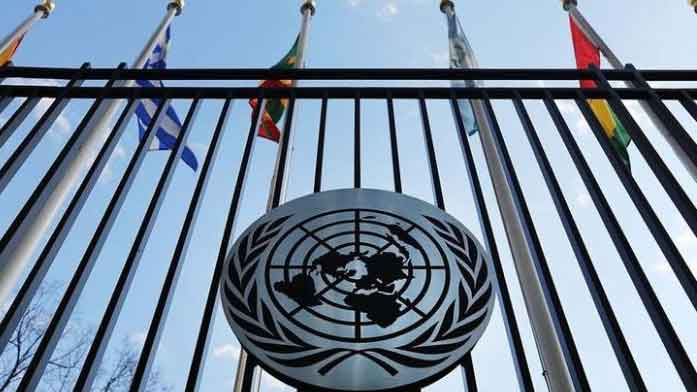
\includegraphics[width=300px]{259.jpg}%
\newline%
%
Ginebra.{-}Las Naciones Unidas liberaron este lunes unos 9,2 millones de dólares para nutrición, atención médica y otro tipo de ayuda para los venezolanos a través de un fondo para ayuda de emergencia.%
\newline%
%
Es la primera ayuda de ese tipo para Venezuela desde que empeoró la crisis política y económica en el país.%
\newline%
%
La decisión de desbloquear el Fondo Central para la Acción en Casos de Emergencia por parte de varias agencias de la ONU, que fue tomada desde mediados de noviembre, representa un pequeño avance debido a que dicho fondo generalmente requiere la aprobación del gobierno del país al que será destinado, reseñó AP.%
\newline%
%
El gobierno de Maduro ha negado en varias ocasiones que Venezuela necesite ayuda externa y ha tratado de responsabilizar de los problemas del país a las naciones que considera como imperialistas, como Estados Unidos y algunos miembros de la Unión Europea%
\newline%
%
La cantidad más reciente, desembolsada el lunes, involucra 2,6 millones de dólares para apoyo nutricional para niños, mujeres embarazadas y madres en periodo de lactancia.%
\newline%
%
\end{document}